\documentclass[10pt,twocolumn,letterpaper]{article}
%\documentclass[10pt,onecolumn,letterpaper]{article}

\usepackage{cvpr}
\usepackage{times}
\usepackage{epsfig}
\usepackage{graphicx}
\usepackage{amsmath}
\usepackage{amssymb}
\usepackage{bbm}
\usepackage{caption}
\usepackage{subcaption}
\usepackage{epstopdf}
\usepackage{multirow}
\usepackage{epigraph}
\usepackage{algorithm2e}


% Include other packages here, before hyperref.

% If you comment hyperref and then uncomment it, you should delete
% egpaper.aux before re-running latex.  (Or just hit 'q' on the first latex
% run, let it finish, and you should be clear).
\usepackage[breaklinks=true,bookmarks=false]{hyperref}

\cvprfinalcopy % *** Uncomment this line for the final submission

\def\cvprPaperID{****} % *** Enter the CVPR Paper ID here
\def\httilde{\mbox{\tt\raisebox{-.5ex}{\symbol{126}}}}

% Pages are numbered in submission mode, and unnumbered in camera-ready
%\ifcvprfinal\pagestyle{empty}\fi
\setcounter{page}{1}

\newtheorem{theorem}{Theorem}
\newtheorem{definition}{Definition}

\begin{document}

%%%%%%%%% TITLE
\title{ Abstraction and Optimization: Applying Multiple Flow Tables in Software Defined Networks}

\author{
Xiaorui Dong, Yukun Zhu\\
University of Toronto\\
{\tt\small xiaorui.dong@mail.utoronto.ca, yukun@cs.utoronto.edu}
%{\tt\small yukun@cs.utoronto.edu}
%Institution1\\
%Institution1 address\\
% For a paper whose authors are all at the same institution,
% omit the following lines up until the closing ``}''.
% Additional authors and addresses can be added with ``\and'',
% just like the second author.
% To save space, use either the email address or home page, not both
%\and
%Second Author\\
%Institution2\\
%First line of institution2 address\\
%{\tt\small secondauthor@i2.org}
}

\maketitle
%\thispagestyle{empty}

%%%%%%%%% ABSTRACT
\begin{abstract}
SDN is one of the most active research fields in computer science discipline. With tons of innovative researches coming each year, current hardware limitations, especially the limited TCAM storage space, are becoming the bottleneck of many state-of-the-art algorithms and designs. Moreover, the growing size of network and the increasing demand for bandwidth also push hardware limitations to a critical section in SDN research. In our project, we aim at designing an efficient and effective architecture that blends fast, expensive TCAM with slow but relatively cheaper SRAM. Our proposed approach could split rules into conflict-free partitions, which preserve the behaviour of the switch and also lead to an abstraction of multiple flow tables. We also propose an optimization algorithm to find the best partition over exponential number of feasible solutions. Experiments in a simulated environment demonstrate the effectiveness of our approach. 

\end{abstract}


%%%%%%%%% BODY TEXT

\tableofcontents

\section{Introduction}\label{sec:1}
The emergence of Software Defined Networks (SDN)\cite{mendonca2013survey} eases the pain in managing networks by having a logically-centralized controller and distributed, configurable flow-based switches. SDN controllers have a global view of the entire network, while applications running on controllers can allocate and optimize the network resources by installing/removing particular rules, which specify  \textit{patterns} to match certain packets and \textit{actions} to manage the matched packets (such as forward, drop, or send to controller). Those rules are typically stored in high-speed memories such as Ternary CAMs (TCAM). Unfortunately, commercial switches can only be equipped with limited high-speed memories due to their high manufacturing cost and high power consumption. In fact, most commercial switches today can only support up to tens of thousands of rules\cite{nakagawa2013domainflow,stephens2012past}.

However, the number of rules increases rapidly with the growing complexity of networks. In addition, the ultimate success of SDN and enabling technologies such as OpenFlow\cite{mckeown2008openflow} motivate programmers to develop various applications to implement, enrich and extend the functionality of networks. Those customized applications might call for more delicate rules to exhaustively fine-tune the entire network, thus the total number of rules might easily go beyond the physical limit of switch resources. OpenFlow specification manages flow table by using per-rule inactivity timeouts to evict rules when they have not been recently accessed\cite{zarek2012openflow}. But it also increases the burden of controllers to install previously evicted rules once necessary.

Researchers have been well aware of the limitations of on switch memories. They have proposed various techniques to select and compress flow-table entries to lower switches memory utilization\cite{curtis2011devoflow,nguyen2014optimizing,yu2010scalable}. Novel flow table structures and multiple flow tables are also proposed to efficiently manage rules\cite{nakagawa2013domainflow}. Inspired by those exciting researches, we would like to design multiple flow tables by combining both high-speed memory units (such as TCAM) and high-capacity memory units (i.e. SRAM). We can further optimize the rule placement in multiple flow tables by analysing the network model. Meanwhile, motivated by how modern operation systems manage virtual memories for each process, we would also like to provide programmers with an abstraction of switch memories. This abstraction will make our multiple flow tables completely transparent for high-level applications.

In the remainder of the report, we first review related work in Section \ref{sec:rw}. In Section \ref{sec:acmft}, we introduce our abstraction for multiple flow tables and explain how we address potential issues in our architecture. Section \ref{sec:opt} gives detailed analysis on the optimization of rule placement in multiple flow tables. Experimental results are illustrated in Section \ref{sec:exp}.

\section{Related Work} \label{sec:rw}


\subsection{TCAM and SRAM}

Ternary content addressable memory (TCAM) is designed specifically for high-speed lookups. Searching in TCAM generally takes a constant time regardless the size of its content, making TCAM an ideal candidate for storing rules in network routers and switches.

However, TCAM does have several disadvantages. TCAM is less dense than SRAM. Even an area-optimized, CMOS-based TCAM cell is over 90 times larger than a DRAM cell at the same technology node, which limits the capacity of commercially available TCAM to a few megabytes\cite{guo2011resistive}. Meanwhile, the comparator’s circuitry in TCAM cell adds complexity to the TCAM architecture. The extra logic and capacitive loading due to the massive parallelism lengthen the access time of TCAM, which is 3.3 times longer than the SRAM access time\cite{dharmapurikar2006longest}. TCAM also consumes significantly more power in both read and write operations \cite{mahoney2005parallel}. Furthermore, TCAM is not subjected to the intense commercial competition found in the RAM market. The cost of TCAM is about 30 times more per bit of storage than SRAM \cite{taylor2005survey}. In contrast, RAM is available in a wider variety of sizes and flavours, is more generic and widely available, and enables to avoid the heavy licensing and royalty costs charged by some CAM vendors\cite{ullahz}.

\subsection{Optimization on Flow Tables} 
Existing studies on OpenFlow rule selection and placement focus on storing the most important rules on special switches, which reduces the workload on controllers. DIFANE\cite{yu2010scalable} caches the most important ones at authority switches, thus that ingress switches will redirect packets which cannot match any rules in current flow table towards authority switches. Similarly, vCRIB\cite{moshref2013vcrib} puts rules in both hypervisors and switches. 

OpenFlow flow table, although flexible in structure, is not hardware friendly, which in turn impacts its scalability. Researchers from Fujitsu\cite{nakagawa2013domainflow} found that commodity switches might contain exact matching tables for the forwarding databases. In order to utilize switch hardware resources efficiently, they propose DomainFlow. DomainFlow solves the limitation by splitting network into two domains. Domain 1 contains the wild-carded matching rules, and domain 2 holds the exact matching rules. DomainFlow significantly reduces the number of entries in the flow table in certain network configurations by using exact matching wherever possible. Also, splitting network into sections helps increase the usage of exact matches.  Meanwhile, Bo \etal proposed a reactive wildcard rule caching system that could handle rule placements to better store wildcard rules \cite{yan2014cab}. Their method allows more wildcard rule to reduce the total number of entries in flow tables, but it also requires fine-tuning on model parameters, and bad parameter selection might result in overwhelming memory spaces.

Another interesting study aims at maximizing the value of the traffic from the actual dimensioning of the network\cite{nguyen2014optimizing}. In this research, they proposed a model with several constraints that can be used to compute the best allocation of rules. Their model is applied to switches with one flow table stored on TCAM, and discards any low-weighted rules once the flow table is fully occupied.  

Our project is inspired by previous researches, but also has a set of important differences. First, our model targets on combination of flow-tables which provides larger capacity for rules in general network configurations. A preliminary idea is that we combine fast, expensive TCAM with slower, cheaper SRAM to build hybrid multiple flow tables. The challenge of implementing this idea lies in how to resolve the conflict among rules generated by various applications, as well as how to address rule priorities. Moreover, we leverage the power of centralized controllers to better allocate those rules. Close scrutiny on corresponding rules in distributed switches might be critical to achieve this goal. Finally, our model should also be orthogonal with certain previous methods \cite{yu2010scalable,curtis2011devoflow} owing to abstraction \textemdash those methods should run on top of our method as if there is only one flow table per switch.


\section{Abstraction for Conflict-free Multiple Flow Tables} \label{sec:acmft}

The benefit of multiple flow tables lies mainly in their large capacity, but it also brings several drawbacks. The threshold issue for concatenated multiple flow tables is their considerable latency if we exhaustively search all flow tables to find the exact rules for a particular incoming flow. Several methods such as pure divide-and-conquer could effectively reduce the search domain for rule matching, but those methods usually rely on a particular structural of flow tables arrangement, and are less likely to preserve high memory space utilization in certain circumstances. Meanwhile, tuning such methods on a given network is often artificial and labour-intensive. 

Another drawback for multiple flow tables is their unfriendly programming interface for network programmers. Assuming we have a perfect system that could intelligently find the right flow table for any incoming flows, will programmers know the details of such operation? Ideally, this perfect system should run transparently from a programmer's view to enable scalability and portability. But transparency also reduces the ability for this system to adapt to different applications and network conditions. 

Although flow table design and management have been studied in depth in many literatures, only a few of them focus on multiple flow tables. In contrast, hierarchical memory management in PC has already been studied for decade, and the key idea so far is to provide programmers a virtual memory for each process, and put the duty of memory optimization to operation systems. Motivated by this solution, our proposed model addresses these two issues by providing a universal strategy to abstract and optimize multiple flow tables. We hide all implementation details of our method from programmers to ensure the scalability and portability of our method. Meanwhile, our model does take input from programmers \textemdash this enables our method to better optimize itself for a particular application.  

\subsection{Abstractions for Two Flow Tables}\label{sec:abs_two}

\textit{Notation.} In this paper we follow standard mathematical notations with a few self-defined types/operations. In particular, $\{T\}$ represents a set containing elements of type $T$, and $\left< T \right> = \left< T_1, T_2, \ldots, T_n \right> $ indicates an ordered list of $T$. $|\cdot|$ operates on a set or ordered list to get its size (number of elements in the set/ordered list). $\{T\} - T_{rm}$ means remove the element $T_{rm}$ from $\{T\}$.   $\emptyset$ represents an empty set or an empty ordered list. In addition, $\{T_1\} \to \{T_2\}$ denotes the set of functions that takes arguments from ${T_1}$ and then maps to elements in ${T_2}$.

We start introducing our method with a simple example, where each switch is equipped with two flow tables. Without loss of generality, we assume one flow table is implemented with fast, expensive TCAM and the other is implemented with large, slow SRAM. For TCAM we have a fixed capacity of $c_t$ and its latency is $\tau_t$ while for SRAM we have $c_s$ and $\tau_s$. We also define matching pattern $m$, which is a finite set of packet headers $h$ and represents the matching information (i.e. a combination of source IP address, destination IP address and port number) for each rule $r=\{m_r, a_r, s_r, p_r\}$, where $m_r \subseteq \{h\}$ is the matching pattern of this rule, $a_r$ is its action, $s_r$ represents collected statistics and $p_r$ is its priority. Our switch will match the header $h$ of each incoming flow to a set of rules $\{r\}$, find the matched rule $r^*$ with highest priority and execute the corresponding action $a_{r^*}$. This process can be modelled as a matching function $S \in h \times \{r\} \to \{\emptyset\}\cup \{a\}$, where $h$ and $\{r\}$ is a particular header and a set of rules, respectively, and $\{a\}$ is the set of  actions after matching the all the rules in $\{r\}$.  $S(h,\{r\})=\emptyset$ if and only if $\forall r' \in \{r\}, h\not\in m_{r'}$. In this paper we generally ignore the statistic field $s_r$ as it doesn't have impact on our abstraction and optimization. 

Assuming both flow tables are full and the frequency of visiting each rule is the same, theoretically, the lowest achievable average latency for this two flow table architecture is $\frac{c_t}{c_s+c_t} \times \tau_t+\frac{c_s}{c_s+c_t} \times \tau_s=\frac{c_s \tau_s + c_t \tau_t}{c_s+c_t}$. In practice, greedily searching the entire flow table space for the best match may reach a space utilization of $100\%$. However, this method also have a latency of $\tau_t+\tau_s$ for every incoming flow, which counteract the benefit of TCAM. Another solution is to apply divide-and-conquer as in\cite{yan2014cab}, a commonly used programming paradigm in the header space. Divide-and-conquer will manually set a partition $\{H_t, H_s\}$, where $H_t, H_s \subseteq \{h\}$ from the hyperspace of $h$, thus that a minimum number of rules are split by $\{H_t, H_s\}$. This partition can be obtained by solving the minimal cut problem on a undirected graph. Any flow with header $h\in H_t$ will trigger lookup in TCAM and that with $h\in H_s$ will search in SRAM. Statistically, this technique will have average latency of $\tau_p+ \frac{c_s \tau_s + c_t \tau_t}{c_s+c_t}$, where $\tau_p$ is the latency in finding the right partition for each flow header. However, finding the right partition that maps each $h$ to $\{H_t, H_s\}$ is computational expensive, and it will also heavily impact the space utilization of this method. Moreover, any rule whose matching pattern $m$ overlaps with both $\{H_t, H_s\}$, that is, any rule that crosses the partition, will be kept in both flow tables. This in turn increases the total size of memory required.

Ideally, our system should keep high space utilization and comparatively low average latency. Inspired by the divide-and-conquer approach, our method adopts a partition in rule spaces $\{R_t, R_s\}$, that is, any rule that belongs $R_t$ should be stored in TCAM and that in $R_s$ is in SRAM. Assuming rules in $\{R_t\}$ and $R_s$ are \textit{independent}, which means the union of all matching patterns of rules in $R_t$ and $R_s$ have empty intersection, then we could search TCAM first to find possible matches. If not found, we then search SRAM and return corresponding action for a particular packet header. If no match is found in both tables, we divert the packet to the controller. In this scheme, we will have an average latency of $\frac{c_t \tau_t + c_s (\tau_s+\tau_t)}{c_s+c_t}$. Consider that $\tau_t \ll \tau_s$, the latency of our system is close to the optimal $\frac{c_s \tau_s + c_t \tau_t}{c_s+c_t}$. Meanwhile, our system could also reach the space utilization of $100\%$.

Although this system looks nice, but we have made an assumption that rules in $R_t$ and $R_s$ are independent. This independence ensures that any packet header $h$ will only match either the rules in $R_t$ or $R_s$. It is very likely that such partition doesn't exist in practice. However, the key constraint of our method is to ensure any match found in TCAM will be final, and this constraint can be satisfied by finding a \textit{conflict-free} partition in rule space. The precision definition of conflict-free partition is given in Def. \ref{def:conflict_free}.

\begin{definition}
\emph{(conflict-free)}
\label{def:conflict_free}
An ordered partition in rule space $\left< R_1, R_2 \right>$ is conflict-free if and only if for any packet header $h$, $S(h,R_1) = \emptyset$ or $S(h,R_1)=S(h,R_1 \cup R_2)$
\end{definition}

Based on Def. \ref{def:conflict_free}, an arbitrary rule set $R$ will always have at least two conflict-free partition, $\left< R, \emptyset \right>$ and $\left< \emptyset, R \right>$. But these partitions are trivial in implementing our multiple flow tables. Unless otherwise specified, in the rest of this paper we regard all conflict-free partition as \textit{non-trivial conflict-free partition}, which ensures $R_1, R_2 \neq \emptyset$.

Another issue of conflict-free partition is that if there will be at least one non-trivial conflict-free partition for a given rule set. Unfortunately, Table. \ref{tab:negative} illustrates such an example.

\begin{table}[h]
\centering
\begin{tabular}{|lc|c|}
\hline
$h$	 &	$\{r\}$	& $S(h,\{r\})$\\
\hline\hline
$h_1$ & $\{r_1\}$    & $a_1$ \\
$h_1$ & $\{r_2\}$    & $a_2$ \\
$h_1$ & $\{r_1,r_2\}$ & $a_1$\\
$h_2$ & $\{r_1\}$    & $a_3$ \\
$h_2$ & $\{r_2\}$    & $a_2$ \\
$h_2$ & $\{r_1,r_2\}$ & $a_2$\\
\hline
\end{tabular}
\caption{An example where no conflict-free partition exists.}\label{tab:negative}
\end{table}

It is easy to prove that no conflict-free partition exists for rule set $\{r_1,r_2\}$ with the given matching function $S$ in Table. \ref{tab:negative} (the only two non-trivial partition $\left< \{r_1\}, \{r_2\} \right>$ and $\left< \{r_2\}, \{r_1\} \right>$ are not conflict-free). This example also demonstrates that seeking a conflict-free partition requires knowledge on matching functions for each packet header. Luckily, those matching functions must satisfy a few constraints listed in OpenFlow standard\cite{mckeown2008openflow}, that is, those functions must be uniquely determined by the matching pattern, action and priority of each rule. That means for each packet header $h$, the set of matched rules $R_m = \{r| S(h,\{r\})\neq \emptyset\}$ will either be $\emptyset$ (no match found for this packet header, divert to controller by default) or have a rule $r^* \in R_m$ such that $\forall r' \in R_m, r' \neq r^*, p_{r^*}>p_{r'}$. The matching function in previous case will be $S(h,R)=\emptyset$ and that in latter case is $S(h,R)=a_{r^*}$, where $R$ is the set of all rules in flow tables. We define the term \textit{stable rule set} for such rule sets as in Def. \ref{def:stable_rule_set}.

\begin{definition}
\emph{(stable rule set)}
\label{def:stable_rule_set}
A rule set $R$ is a stable rule set if and only if $\forall h$, either $\forall r \in R, h\not\in m_r$ or $\exists r^* \in R$, such that $h \in m_{r^*}$ and $\forall r' \in R, r'\neq r^*, h\in m_{r'}, p_{r^*}>p_{r'}$. 
\end{definition}

The property of stable rule set casts several constraints on the matching function $S$ in all single-valued function in $h \times \{r\}$. In this paper, we also safely assert all the rules in a given switch or router should always form a stable rule set. However, will there always exist a conflict-free partition for any stable rule set? Will the conflict-free partition for the stable rule set to be unique? How to find a conflict-free partition in all possible partitions (the total number of partitions increases exponentially with the number of rules)? We will address those issues by constructing a conflict-free partition $\left< R_1, R_2 \right>$ on a given stable rule set $R$.

We first define \textit{overlap} $(\oplus)$ as a binary relationship between arbitrarily two rules $r_X$ and $r_Y$ in Eqn. \ref{eqn:overlap}. 

\begin{equation}
\begin{split}
	\oplus := \{&(r_X,r_Y) | m_{r_X} \cap m_{r_Y} \neq \emptyset  \land \exists h \in m_{r_X} \cap m_{r_Y},\\ & S(h,\{r_X\}) \neq S(h,\{r_Y\})\}\label{eqn:overlap} 
\end{split}
\end{equation}


In Eqn. \ref{eqn:overlap}, any rules that overlap will have a non-empty intersection in their matching pattern and different action. We further define another binary relationship \textit{stronger than} $(\succ)$ as in Eqn. \ref{eqn:stronger}

\begin{align}
	\succ := \{&(r_X,r_Y) | r_X \oplus r_Y \land p_X>p_Y \\
	&\land \exists h\in m_{r_X}\cap m_{r_Y}, S(h,\{R\})=a_{r_X} \}\label{eqn:stronger} 
\end{align}

The binary relationship $\succ$ is asymmetric but not transitive. We then propose an algorithm to construct the conflict-free partition $\left< R_1, R_2 \right>$ as in Alg.\ref{alg:greed}.

\begin{algorithm}[h]
\KwData{a stable rule set $\{R\}=\{r_1,r_2,\ldots, r_n\}$, and desired size $C_{R_1}$ for $R_1$\;}
\KwResult{a conflict-free partition $\left< R_1, R_2 \right>$, $R_1 \neq \emptyset$, $|R_1| \leq C_{R_1}$, $R_1 \cup R_2 = R$\;}
\textbf{init:} set $R_u=\{\{r_i\},i\in [1,n]\}$, graph $G = (V,E)$ such that $V=R$ and $(r_i,r_j)\in E \iff r_i \succ r_j$\;

\While {$E \neq \emptyset$}{
	randomly pick $e=(r_{k1},r_{k2})\in E$, $E := E - {e}$\;
	
	\If{$\not\exists {r'}\in R_u, r_{k1},r_{k2} \in r'$}{
		merge $\{r_a\}, \{r_b\}$ in $R_u$, where $r_{k1}\in\{r_a\}$ and $r_{k2}\in \{r_b\}$\;
	}
}
\While {$|R_1|<C_{R_1}$ and $\exists \{r\}\in R_u$ such that $|\{r\}|\leq C_{R_1}-|R_1|$}
{
	$R_u := R_u - \{r\}$; $R_1 := R_1 \cup \{r\} $\;
}
\If {$|R_1|<C_{R_1}$}
{
	randomly select $\{r\} \in R_u$, move $C_{R_1}-|R_1|$ rules with top priority to $R_1$\;
}
$R_2 = R\backslash R_1$\;
\caption{Algorithm for constructing conflict-free partition}
\label{alg:greed}
\end{algorithm}

We can easily prove that the constructed partition $\left< R_1, R_2 \right>$ is conflict-free by contradiction. Given the fact that $R_1$ and $R_2$ are stable rule sets, if $\exists h$ such that $S(h,R_1)\neq S(h,R_1 \cup R_2)$ and $S(h,R_1)\neq \emptyset$, there must be a rule $r^*\in R_1 \cup R_2$ such that $\forall r' \in R_1 \cup R_2, r'\neq r^* $ and $ h\in m_{r'}$, $p_{r*}>p_{r'}$. In this case, $S(h,R_1 \cup R_2)=a_{r^*}$. As $S(h,R_1) \neq a_{r^*}$, that is to say, $r^* \in R_2$ and $\exists r'', r''\neq r^* $, $ r''\in R_1$ and $h\in m_{r''}$. This implies $r^*\succ r''$ As our algorithm will initialize $(r'',r^*)\in E$, $r^*$ and $r''$ should be in the same set after the while loop in Alg. \ref{alg:greed}, and $r^*$ and $r''$ will either both be in $R_1$ or $R_2$, or $r^* \in R_1$ and $r'' \in R_2 $ as $r^*$ has higher priority. That contradicts with our assumption that $r^* \in R_2$ and $r'' \in R_1$.

\subsection{Abstractions for Multiple Flow Tables}
In Sec. \ref{sec:abs_two}, we build a two flow table architecture and design a conflict-free partition in rule space that could resolve the conflict with two flow tables. In this section, we will extend our architecture to multiple flow tables.

\begin{theorem}
For a stable rule set $R$ and integer $N\leq |R|$, there will always be a conflict-free partition $\left<R_1,R_2,\ldots,R_n\right>$ with size $C_{R_1},C_{R_2},\ldots,C_{R_n}$ such that $|R|=sum_{i=1}^n C_{R_i}$ and $C_{R_i}>0$.
\end{theorem}

This theorem follows naturally with our algorithm Alg. \ref{alg:greed}. As the first part of our algorithm is basically trying to find all the connected component in the giving graph $G$ and the second part is trying to randomly allocate connected component to $R_1$, we can iteratively assign multiple sets $R_1,R_2,\ldots,R_n-1$ in a similar manner. However, multiple flow tables is able to provide additional features to our architecture (\eg we could build a rapid hash table in SRAM for exact match only; we can also optimize forwarding decision making process as in \cite{shelly2014flow}). 

Another method that could boost the performance of our method is to do multi-thread matching. As all the flow tables in our architecture are independent, \ie we don't specify inter-table relationships, we could simultaneously search all the flow table at the same time. Once we find a match in a certain flow table and searches are over in all previous tables, we can safely stop all threads and analyse returned matches. Assuming all the flow tables are ranked by ascending latency $\tau_i$, and their capacity are $c_i$, our architecture could reach $\frac{\sum_i c_i\tau_i}{\sum_i c_i}$ with multi-threading. Reduced to the cases with only two flow tables, that is exactly the lowest average latency we could achieve.

\section{Optimization} \label{sec:opt}
An important observation from Alg.\ref{alg:greed} is that our generated partition might not be unique. Meanwhile, our statistical analysis assumes the matching frequency of each rule is evenly distributed, and that is an oversimplified assumption in real-world scenario. Moreover, our abstraction is totally transparent for programmers, that enables portability but also  prevents fine tuning and optimization. Those factors motivate us to find a rule to optimize our partitions, or, to find the best partition in all possible conflict-free partitions.

We first reduce our abstraction to a two-flow-table architecture. In this case, we would like to find the best partition $\left<R_1,R_2\right>$. To allow programmers tuning our architecture, we set a hyper-parameter $\omega=[\omega_1,\omega_2]$ in our model. $\omega_1$ is a vector that indicates the bonus associated with putting rules in $R_1$ and $\omega_2$ is the bonus of storing rules in $R_2$. This $\omega$ depends only on the application developers. For the $i^{th}$ rule, we should expect $\omega_1(i)\geq \omega_2(i)$ as putting rules in the first table is always favourable.

We further define binary random variable $f_i$ and $g_i$ as indicator variables. $f_i=1$ indicates $i^{th}$ rule should be put in $R_1$ and $g_i=1$ for $R_2$. Given those definitions, our optimization problem can be written as in Eqn. \ref{eqn:obj}.

\begin{align}
f_i^*,g_i^*=\arg\max_{f_i,g_i}\mathcal{O}= \arg\max_{f_i,g_i}\sum \omega_1(i)f_i + \omega_2(i)g_i \label{eqn:obj}
\end{align}

Eqn. \ref{eqn:obj} is the linear objective function of our optimization problem. As the indicator variables are constrained by forming a conflict-free partition, and our measure over rule space in Eqn. \ref{eqn:stronger} is asymmetric but not transitive, inference of our model is basically maximize the objective function over a directed acyclic graph. We will discuss the constraints for the indicator variables in the following sections.

\subsection{Optimization with Local Cues}
In this section, we mainly concentrate on optimization on a single switch. Generally, we have the following constraints for our indicator variables.

\begin{align}
\label{eqn:con1}\forall i, f_i, g_i &\in \{0,1\} \\
\label{eqn:con2}\forall i, f_i+g_i &\leq 1 \\
\label{eqn:con3}\forall i,j, r_i \succ r_j \to f_i-f_j &\geq 0 \\
\label{eqn:con4}\sum_i f_i &\leq C_{R_1} \\
\label{eqn:con5}\sum_i g_i &\leq C_{R_2}
\end{align}

With the objective function in Eqn. \ref{eqn:obj}, this forms an integer programming (IP) problem. Here constraint \ref{eqn:con1} ensures all the variables are boolean and constraint \ref{eqn:con2} specifies a rule should be placed on either sets($R_1$ or $R_2$). Constraint \ref{eqn:con3} keeps stronger rules to be in the same table, or the higher table than other rules. Constraint \ref{eqn:con4} and \ref{eqn:con5} enforce capacity limits for both tables. For this IP formulation, we could prove the following theorem holds for stable rule sets:

\begin{theorem}
The solution space for our IP formulation is the set of all conflict-free partition subject to $|R_1|\leq C_{R_1}$. 
\end{theorem}

We can prove this theorem by proving all conflict-free partition shares above properties, and the solution satisfying those constraints constructs a conflict-free partition. For the first part, \ref{eqn:con1} and \ref{eqn:con2} will always hold as a particular rule can only be in $R_1$ or $R_2$. And Eqn. \ref{eqn:con1} \ref{eqn:con4} specifies the capacity constraint. If $\exists$ conflict-free partition $\left<R_1,R_2\right>$ such that $\exists i,j, r_i \succ r_j$ and $f_i<f_j$, then we have $f_i=0$ and $f_j=1$. That implies $r_j \in R_1$ and $r_i \in R_2$. So $\exists h\in m_{r_i}\cap m_{r_j}$, $S(h,R_1 \cup R_2)=a_{r_i}$ and $S(h,R_1) \neq a_{r_i}$, which contradicts with our assumption that $\left<R_1,R_2\right>$ is conflict free.

For the second part, as stronger rules will at least be in the same table as ordinary rules, there will never be the case where a lower priority rule takes effect in $R_1$ while the one with higher priority lies in $R_2$. That guarantees to construct a conflict-free partition.

\subsection{Optimization with Global Information}
The main power of SDN lies in its centralized controller. This controller knows the topology and configuration of the entire network, thus we could better optimize our scheme with global information. 

In this formulation, we are interested in a picture of the entire network. Now we rewrite the indicator variable as $f_{i,s}$ and $g_{i,s}$, where $s$ indicates the switch where this rule locates. Our objective function will be as in Eqn \ref{eqn:obj2}.

\begin{equation}
f_{i,s}^*,g_{i,s}^*=\arg\max_{f_{i,s},g_{i,s}} \sum_{s}\sum_{i=1}^{N_s} \omega_1(i)f_{i,s} + \omega_2(i)g_{i,s} \label{eqn:obj2}
\end{equation}

Here $N_s$ denotes the total number of rules on switch $s$. All the local constraints still preserves, and we rewrite them as follows:

\begin{align}
\label{eqn:con1b}\forall i,s, \quad f_{i,s}, g_{i,s} &\in \{0,1\} \\
\label{eqn:con2b}\forall i,s, \quad  f_{i,s}+g_{i,s} &\leq 1 \\
\label{eqn:con3b}\forall i,j,s, \quad  r_{i,s} \succ r_{j,s} \to f_{i,s}-f_{j,s} &\geq 0 \\
\label{eqn:con4b}\forall s, \quad  \sum_i f_{i,s} &\leq C_{R_1,s} \\
\label{eqn:con5b}\forall s, \quad  \sum_i g_{i,s} &\leq C_{R_2,s}
\end{align}

In addition, we also would like to encourage a coordinated behaviour across the network. For frequent, important flows, we try to put them in the fast table if there is still space, and we also want to ensure all successor switches could put them in the fast table. We achieve this goal by two different schemes.

\textbf{hard-capping:} In this scheme, if we set a rule $r$ to fast table, its successor switch must keep the matched rule for all the packet headers $h \in m_r$ in the fast table. That can be written as the following constraint.

\begin{align}
\forall (j,s_2) \in successor(i,s_1) \quad f_{j,s_2} \geq f_{i,s_1}
\end{align}

Here $successor(i,s_1)$ indicates the next hop of rule $r_i$ in switch $s_1$ and the corresponding rule is $r_j$. This hard capping method force all successor switch to set matched rule to fast table if it is done so in the previous switch, but might jeopardize performance ahead of a heavily loaded switch.

\textbf{soft-penalizing:} We also adopt a soft-penalizing scheme to enforce coordination between switches and avoid pushing switches too hard. In this scheme, our objective function are as in Eqn. \ref{eqn:obj3}

\begin{align}
\label{eqn:obj3} f_{i,s}^*,g_{i,s}^*=\arg\max_{f_{i,s},g_{i,s}} \sum_{s}\sum_{i=1}^{N_s} \omega_1(i)&f_{i,s} + \omega_2(i)g_{i,s} -C \xi_{s,i}\\
\forall (j,s_2) \in successor(i,s_1) \quad \xi_{s_1,i} &\geq f_{i,s_1} - f_{j,s_2}\\
\xi_{s,i} &\geq 0
\end{align}

In this scheme, we penalize constraint violation in hard-capping scheme by a constant value $C\geq 0$. Setting $C = \infty$ will obtain the same result as hard-capping, and $C=0$ indicates not enforcing coordination constraint. In practise we find an intermediate value, such that we will still allow subsequent switches to put $f_{j,s_2}$ in $R_{2,s_2}$ if by doing so we could put a rule $r'$ in $R_{1,s_2}$ and our objective value increases. This soft-penalizing method contributes most once we have a rule $r_i$ in $s_1$ with high bonus $\omega_1(i)$ and $successor(i,s_1)$ has multiple entries in $s_2$. It might not be efficient to store all its successor in $R_{1,s_2}$ if $(j,s_2)$ have smaller bonus than other rules.   

\subsection{Online Optimization}
Our IP formulation enables programmers to tune our abstraction for two-flow-table architecture, but solving IP, even all its variables are just binary variables, is still a NP-hard problem. Exhaustively searching for the best solution might still be feasible if we only consider local information. However, for a huge network with hundred thousands of nodes/switches, the complexity of our IP formulation will grow exponentially thus brute-force search might not be applicable.

Even though we have an oracle program that could find a exact, or approximate solution for our IP in polynomial time, it might still be inefficient to recompute each solution every time we have a new rule installed. The network is a dynamic system thus we would like to propose an online optimization to effectively place installed rules as quickly as possible. 

One key to achieve online optimization is the observation from Alg. \ref{alg:greed}. As the first step of Alg. \ref{alg:greed} is essentially computing the connected component, and all the connected components are independent with each other in constructing the conflict-free partition, we could separate the formulation into several sub-problems for each connected component, if we only consider local constraints.

Followed by this observation, it is also possible to recompute a small portion of IP once we have an incoming rule. For every new rule $r_{ni}$, we first find all its connected components $\{cc_i\}$. Here $\{cc_i\}$ is a set as $r_{ni}$ could combine multiple disjoint connected components into one. Then we only optimize our model on $\cup_{i}\{cc_i\}$ while fixing all other variables to existing solutions. This recomputing scheme might not find the global maximum but it is guaranteed to converge in a local maximum.

As it is still intractable to optimize rule placements with regard to global constraints, a practical method to apply optimization on a dynamic network is to do online optimization for local constraints only, and the controller will only do network-wide optimization once for a fixed time interval. 

\section{Experiment} \label{sec:exp}
In this section we briefly describe our testbed and simulation environment such as topology, number of switches, applications and \etc. 

\subsection{Experiment Setup}

\begin{figure}[ht!]
\centering
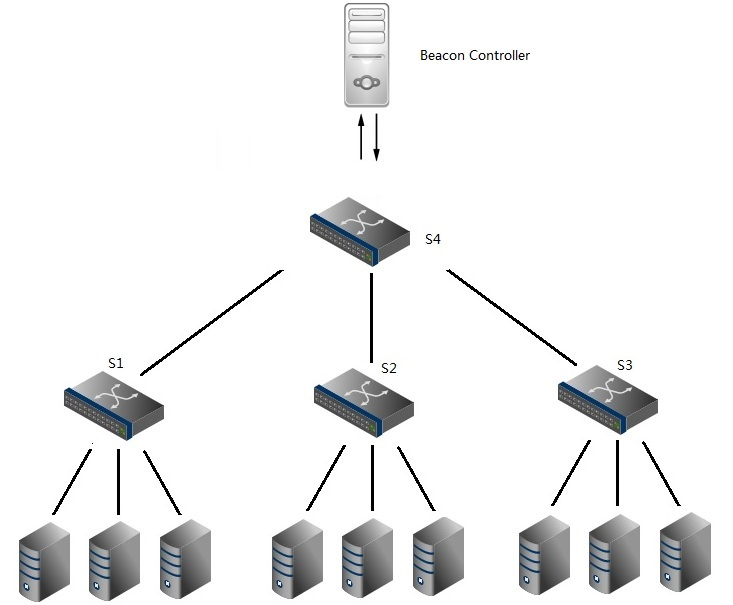
\includegraphics[width=50mm]{Topology.jpg}
\caption{Topology used in our experiment\label{overflow}}
\end{figure}

Numerous controllers rise in the OpenFlow ecosystem. Those controllers are written in diverse languages such Java and Python. According to the published performance comparison, Beacon 1.04 is the most suitable controller for in our experiment. The environment was set up on Virtual Box 4.3.18 with Mininet 2.1.0 on Ubuntu 14.04. For the topology, we created a network with a tree structure. There were 9 hosts, 4 switches, 1 controller in total. Switches composed a two-layer structure. For bottom switches, each one connected 3 hosts. The other switch was sitting on the top of those three switches. Our topology is shown in the Figure 1.

\begin{figure}[ht!]
\centering
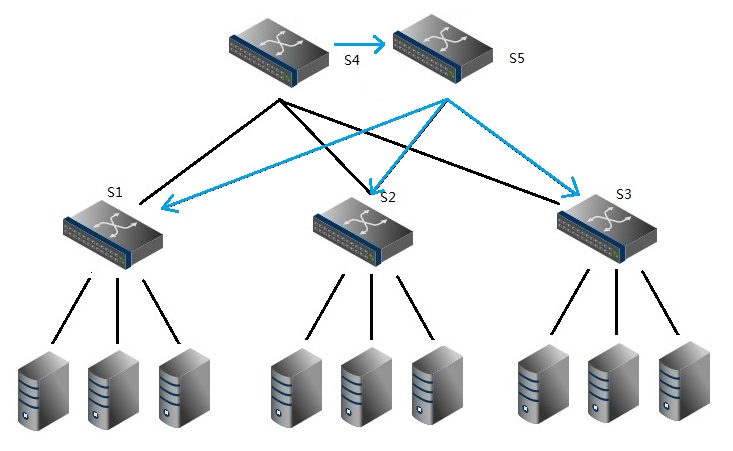
\includegraphics[width=50mm]{TopologyMultilevel.jpg}
\caption{Topology for simulation \label{overflow}}
\end{figure}

The controller application that we used was a level 2 learning switch. Mininet connected the remote controller which was running on the host machine in parallel. As Mininet was running, the l2 learning switch installed exact mating rules to each switches. In the experiment, we set the rules expire time to be infinite. Hence, we could keep using those installed rules. After the flow tables reached a stable stage, we stopped the remote Beacon controller. The stable stage means that no unknown packets were coming. Since flows are matched based on rules' priority, and exact matching rules have default higher priorities than wildcard rules, we removed exact matching rules from the top switch. Then, on the top switch, we installed wildcard rules which contained conflicts, and the traffic among hosts was still alive. At this stage, we let hosts send packets to each other. Then, we recorded the total pass-through packets for each rules on the top switch. Based on each rules’ frequency of usage, we applied our algorithm to split the rule set on the top switch into several conflict-free rule sets. A conflict-free rule set means that rules within the set do not have overlapping with each other. Those rule sets were installed on TCAM and SRAM respectively. In our experiment, we had some limitations since we could not get access to the hardware. Therefore, we simulated them by replacing the top open virtual switch with two switches. One stood for TCAM, and the other represented SRAM. As shown in the Figure 2, S4 is TCAM, and S5 is SRAM. In the topology, we forced packets only to be to access S4, not S5. These two switches could still be considered as one single switch from the hosts and the other switches' perspective. We let the hosts send the packets again, and record the pass-through packets on the simulated TCAM and SRAM respectively. The packets sent from the host were controlled by us. Therefore, we deployed the same packets for both the one-layer flow table and two-layer flow table. Through the experiment, we got an overview of how well our two-layer flow table works.

\subsection{Experiment Analysis}

\begin{figure}[ht!]
\centering
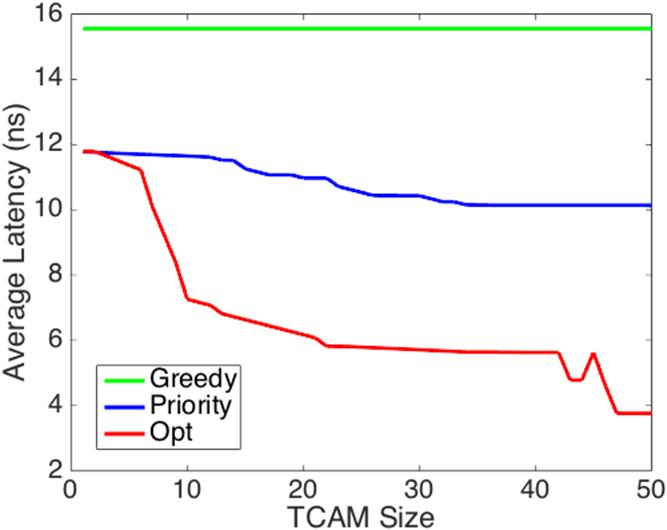
\includegraphics[width=50mm]{ExperimentResult.jpg}
\caption{Simulation Result \label{overflow}}
\end{figure}

In our experiment design, we had three testing scenarios. First one was greedy searching which searched both the TCAM and SRAM. In our case, the one-layer flow table used in Figure 1 stood for this situation. The green line in the Figure 3 is the performance of the greedy algorithm. Then, we sorted the rules on the top switch by priority. Then, we split them into two separate rule sets. Rules which had higher priorities did not mean that they got more frequently used. In the performance chart, the priority sorting did achieve a better result. In the end, we applied our own algorithm to split rules into TCAM and SRAM. As we can see in the chart, the performance is far better than the other two scenarios. However, our experiment was designed for the static environment which means there was no unknown packet. Therefore, the rules installed in the topology were unchanged.

\section{Conclusion} \label{sec:con}
In this paper, we propose an efficient and effective method to expand the storage space on switches by employing multi-layer flow tables. Experiments in simulated environment demonstrate the effectiveness of our method in a static condition. Our proposed method increases the number of rules that a switch can hold, and also minimizes the trade-off of using slower memory medium. We believe our abstraction and optimization can be further improved in a dynamic environment \textemdash a smarter controller that could evaluate and update the rules while handle incoming flows in real-time. 

{\small
\bibliographystyle{ieee}
\bibliography{egbib}
}

\end{document}
